%!TEX root = ../Master Thesis.tex

\chapter{Szenario} % (fold)
\label{cha:szenario}

Für die Master Thesis ist es notwendig, dass ein Szenario existiert, anhand dessen eine Anwendung mit dem MIAV Framework entwickelt werden kann. Da das Framework bisher nur als Modell existiert, muss das Szenario sowohl die Anwendung berücksichtigen als auch die Verwendung des Frameworks. Diese erste Version soll dazu als eine Grundlage dienen, die kontinuierlich weiter entwickelt werden muss.

\section{Rahmen des Szenarios} % (fold)
\label{sec:rahmen_des_szenarios}

Bei dem Szenario handelt es sich um eine Lehrveranstaltung, die \textbf{gleichzeitig} an zwei unterschiedlichen Abteilungen der Fachhochschule Köln stattfindet. Dabei ist aber nicht etwa ein Standort der Sender und der andere entsprechend der Empfänger. Zwischen beiden Standorten herrscht eine bidirektionale Verbindung und Interaktionen sind durch Teilnehmer an beiden Standorten möglich und erwünscht.

% section rahmen_des_szenarios (end)

\section{Beschreibung des Szenario} % (fold)
\label{sec:beschreibung_des_szenario}

An der Fachhochschule Köln - Abteilung Gummersbach findet seit diesem Semester das erste Mal die Veranstaltung "`Medienrezeption"' in einer ganz neuen Form statt. Die Idee die dazu geführt hat ist, verwandte Fachbereiche an der Hochschule auch Standortübergreifend besser zu integrieren. Als Pilotprojekt wurde entschieden, dass die Veranstaltung "`Medienrezeption"' auch von den Studenten des Studiengangs "`Medientechnik"' besucht werden kann. Dieser Studiengang wird am Standort Deutz angeboten. Nun ist die Wahrscheinlichkeit sehr gering, dass die Studenten aus Deutz nach Gummersbach wegen diesem einen Fach fahren, egal wie interessant es auch sein mag. Zudem kommen Koordinationsschwierigkeiten mit dem Stundenplan hinzu. Als Lösung wurde ein einfaches Setup installiert, was eine aktive Teilnahme der Studenten beider Standorte an der Veranstaltung erlaubt:

\begin{itemize}

	\item In jedem Standort sind zwei hochauflösende Webcams installiert, eine die den Dozenten zeigt, eine die das Auditorium zeigt.
	\item In jedem Standort sind zwei Beamer installiert, einen für die Bildinformationen des anderen Standortes und einen für die Folien des Dozenten oder der Studenten.
	\item In jedem Standort ist ein Rechner installiert, über den die Kommunikation realisiert wird.
	\item Die Laptops der Studenten oder des Dozenten werden bei Bedarf an den jeweiligen Kommunikationsrechner angeschlossen, der sämtliche Datenübertragung realisiert.
	\item Die Dozenten erhalten ein eigenes Mikrofon und es stehen 2-3 Mikrofone für die Aufzeichnung der Studenten bereit.
	\item Jeder Standort verfügt über ein Lautsprechersystem.

\end{itemize}

Weitere Punkte die möglich wären:
\begin{itemize}

  \item Hinzufügen der Möglichkeit den Diskurs zu dokumentieren und dann auch mglw. zu persistieren. (Dokumentation/Kommentare via XMPP denkbar?). Nachrichten können dann mit dem Video-/Audiosignal synchronisiert werden.
  \item Es könnten auch weitere Dokumente live bereitgestellt werden. Oder es kann auf Web-Ressourcen verwiesen werden (am einfachsten auch via XMPP).
  \item Der Datenkanal der Laptops könnte statt dem VGA-Signal wirklich die Daten transportieren. Statt also ein Videosignal eines PDF-Dokuments zu schicken, könnte das PDF selbst geschickt werden. Eine Beschränkung auf PDF würde im ersten Schritt reichen. Allerdings muss dann auch die Frage gestellt werden in wie weit die Kontrolle über das PDF geregelt wird: Wer darf scrollen? Wer darf kommentieren? Können die Studenten unabhängig scrollen und kommentieren? Werden diese Kommentare dann live wieder bereit gestellt? Wie sieht die Persistierung dieser Kommentare aus?
  \item Wenn diese reichhaltigen Informationen abgelegt werden, muss es auch eine Möglichkeit geben sie wieder zu finden.

\end{itemize}

Die Veranstaltung "`Medienrezeption"' findet erfahrungsgemäß im kleinen Kreise statt, da es sich um ein Fach im Masterstudiengang handelt. Etwa 10 Studenten der Medieninformatik besuchen sie. Bei den Medientechnikern wird es nicht als Pflichtfach, sondern als Wahlpflichtfach angeboten, daher nehmen in der Pilotphase nur 5 Studenten aus Deutz teil.

Es wird für dieses Setup keine außergewöhnliche Technik benötigt, was die Umsetzung deutlich vereinfacht. Bei allen Komponenten handelt es sich um "`Consumer"'-Artikel, wie man sie in jedem Elektronikmarkt erhalten kann. Lediglich die Verwendung von zwei Beamern ist etwas kostspieliger. Die gesamte Steuerung und Kommunikation wird durch die Applikation auf den Kommunikationsrechnern geregelt, die auf dem MIAV-Framework basiert. Bei den Rechnern handelt es sich ebenfalls um Standard Hardware.

Die Applikation übernimmt unterschiedliche Aufgaben bei diesem Anwendungsfall, so wird von ihr zum einen das Bild beider Kameras zu übertragen zum anderen auch das Signal der jeweils angeschlossenen Rechner. Zusätzlich wird das Audiosignal der Mikrofone übertragen. Die Darstellung des Computersignals erfolgt dabei synchron zu der Darstellung des Videosignals. Die Lautstärke der Mikrofone wird von der Applikation automatisch so angepasst, dass der aktuelle Sprecher optimal zu hören ist und nur wenig Umgebungsgeräusche übertragen werden.

Was ebenfalls von dem System umgesetzt wird, ist das "`Zeigen"' auf Inhalte, die von den Rechnern der Dozenten oder Studenten kommen. Dies wird einfach dadurch realisiert, dass das komplette Videosignal abgegriffen und übertragen wird. Somit also auch der Mauszeiger. In weiteren Versionen wären hier sicherlich intelligentere Methoden denkbar.

  In Abbildung~\ref{fig:images_Hardware_und_Kanaele} sind Kanäle sowie die Hardware dargestellt, so wie sie im Szenario vorkommen.

\begin{figure}[ht]
  \centering
    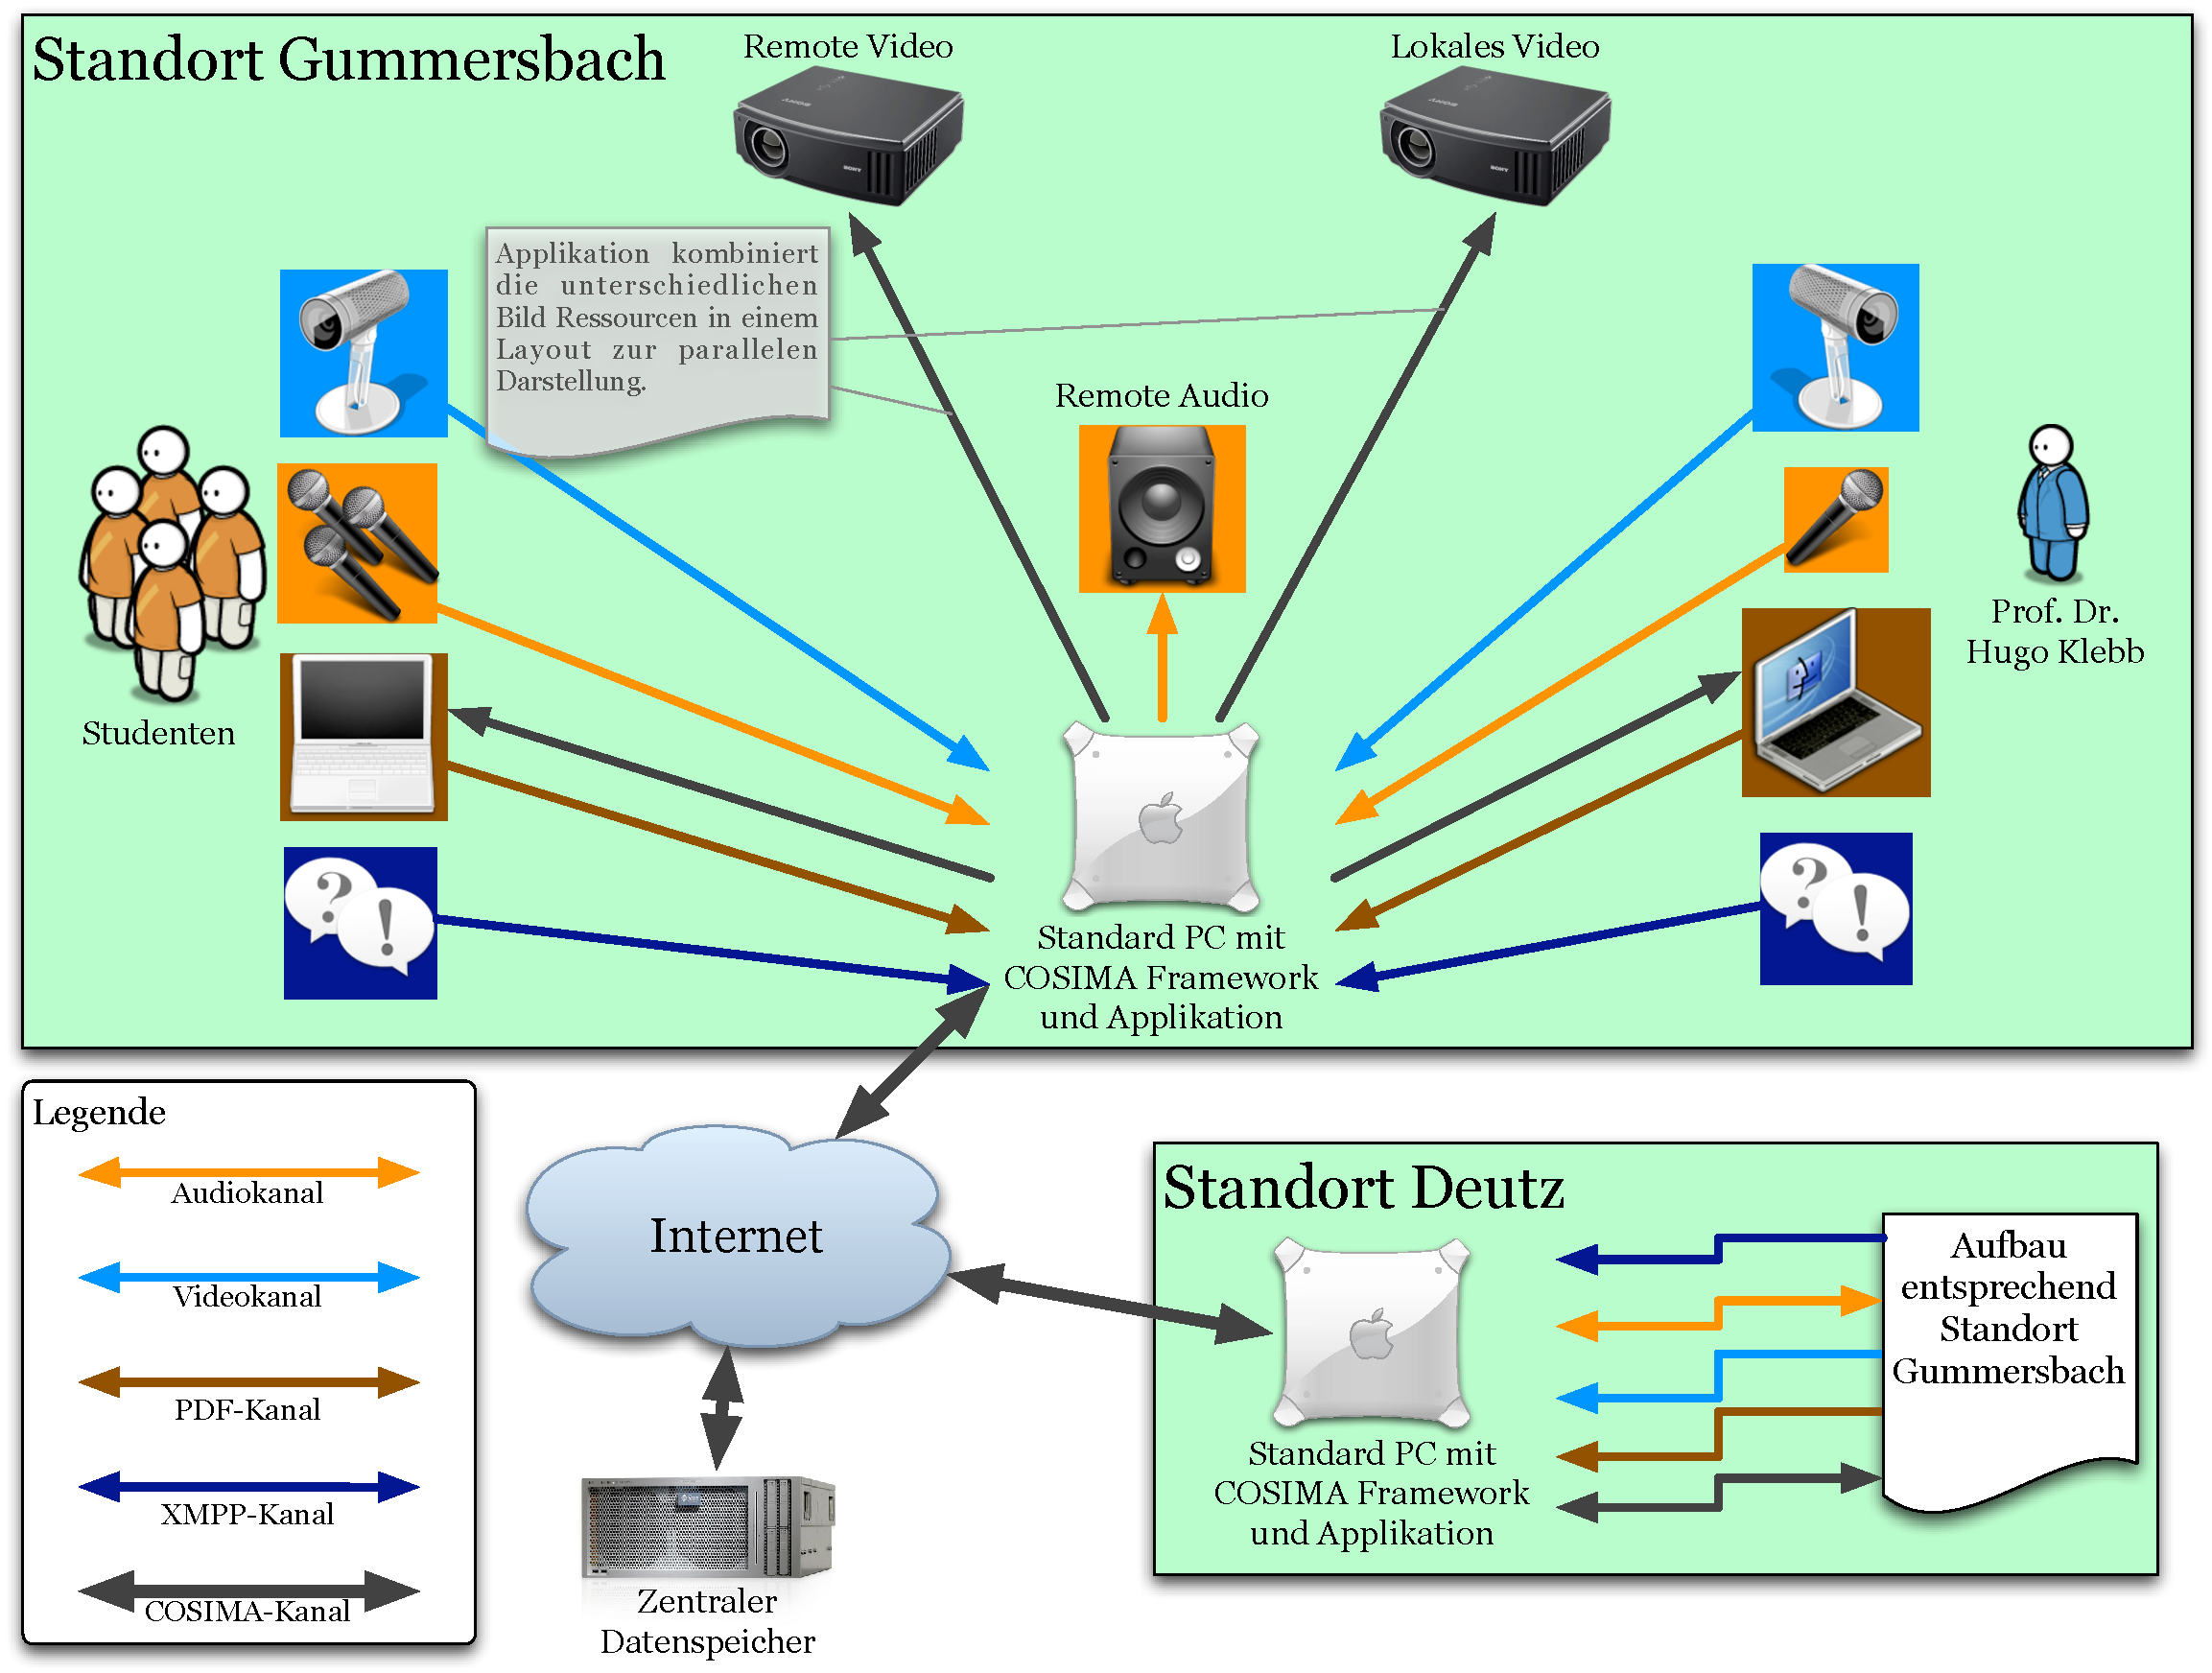
\includegraphics[width=.9\textwidth]{images/Hardware_und_Kanaele.pdf}
  \caption{Diagramm der verwendeten Hardware und Kanäle im Szenario}
  \label{fig:images_Hardware_und_Kanaele}
\end{figure}


% section beschreibung_des_szenario (end)

\section{Ablaufbeschreibung mit Personae} % (fold)
\label{sec:ablaufbeschreibung_mit_personae}

  Es ist ein sonniger Mittwoch vormittag und die Studenten des Masterstudiengangs der Medieninformatik finden sich pünktlich um 09:10 vor dem Raum 3324 an der FH Gummersbach ein. Heute steht "`Medienrezeption"' auf dem Plan. Prof. Dr. Hugo Klebb ist bereits anwesend, da er noch einige technische Vorbereitungen treffen muss. Die Veranstaltung wird zusammen mit Studenten des Studiengangs Medientechnik aus Deutz stattfinden. Das besondere dabei ist, dass die Studenten nicht körperlich anwesend sein werden, sondern durch ein neues System virtuell an der Veranstaltung teilnehmen.
  
  Kurz nachdem sich alle gesetzt haben, steht auch schon die Videoverbindung nach Deutz. Der eine Beamer zeigt ein Videobild von Prof. Dr. Julius Largo, dem Dozenten der Medientechniker und ein weiteres Videobild der Deutzer Studenten. Ebenfalls wird das Computersignal aus Deutz an die Wand geworfen. Auf einem anderen Beamer sehen die Studenten bereits die Folien von Professor Klebb.
  
  Nachdem nun alle Studenten anwesend sind und die Verbindung zwischen den Abteilungen Gummersbach und Deutz steht, beginnt die Veranstaltung. Aufgabe für heute war die Vorbereitung eines Artikels. Jeder Student sollte zu dem selben Artikel eine Textanalyse durchführen. Die Ergebnisse werden bereits im Vorfeld Online den anderen Studenten zur Verfügung gestellt, so dass jeder über das Material des anderen verfügt. Die Veranstaltung ist als seminaristischer Unterricht ausgelegt, es gibt also keinen klassischen "`Frontalunterich"'. Ziel ist es bei der Diskussion über den Artikel ein tieferes Verständnis von der Thematik zu erhalten.
  
  Die Studenten haben alle Laptops dabei und "`klinken"' sich ins FH Netz ein. Jeder kann sich in einen speziellen Chat-Raum einklinken, der nur für diese Veranstaltung gedacht ist. Sie können so parallel zu dem normalen Geschehen, weitere Punkte diskutieren oder dokumentieren. Außerdem steht ihnen auf ihrem Laptop die Möglichkeit zur Verfügung die bisherige und vergangene Veranstaltungen noch einmal anzusehen. Von dieser Möglichkeit macht denn auch direkt Vanessa gebrauch, die etwa 15 Minuten zu spät kommt. Sie stand noch im Stau auf dem Weg nach Gummersbach. Sie klingt sich in das System ein und scannt schnell über die Chat Logs, um zu sehen ob ihr etwas wichtiges entgangen ist. Zum Glück ist dem nicht so und sie kommt schnell wieder in die Veranstaltung rein.
  
  Während der Veranstaltung haben die Studenten den Text über den gesprochen wird ebenfalls auf ihren lokalen Rechnern verfügbar. Allerdings nicht einfach über das Dateisystem, sondern über die Applikation selbst. So können sie das PDF annotieren und diese Annotationen den anderen Studenten wieder zur Verfügung stellen. Auch die Textanalysen der anderen Studenten stehen ihnen über dem selben Kanal zur Verfügung.
  
  [...]
  
  Am Ende der Veranstaltung entsteht so eine Version des Textes, der von allen mit Kommentaren angereichert wurde und Querverweise zu den einzelnen Textanalysen aufweist. Zusätzlich existieren dediziert markierte Punkte im AV-Strom der Veranstaltung, die wieder auf bestimmte Textstellen linken. Angereichert mit den Chat-Logs ist so ein sehr reichhaltiges Ergebnis entstanden, auf das die Studenten und Dozenten auch später immer wieder zugreifen können.
  
\subsection{Personae} % (fold)
\label{sub:personae}

\paragraph{Dozenten} % (fold)
\label{par:dozenten}

  Die Personaebeschreibungen der Dozenten:

  \begin{itemize}

  	\item Prof. Dr. Julius Largo (Deutz)
  	\item Prof. Dr. Hugo Klebb (Gummersbach)

  \end{itemize}

% paragraph dozenten (end)

\paragraph{Studenten} % (fold)
\label{par:studenten}

  Die Personaebeschreibungen der Studenten aus Gummersbach:
  
  \begin{itemize}

  	\item   Thorsten Sommer
  	\item   Vanessa Bergmann
  	\item   Katrin Schreiber
  	\item   Uwe Gaertner
  	\item   Swen Reinhard
  	\item   Anna Müller
  	\item   Ines Gruenewald
  	\item   Nicole Eiffel
  	\item   Sara Kaiser
  	\item   Alexander Feierabend

  \end{itemize}
  
  Die Personaebeschreibungen der Studenten aus Deutz:
  
  \begin{itemize}

  	\item   Barbara Fenstermacher
  	\item   Marina Beike
  	\item   Jennifer Werner
  	\item   Christin Koehler
  	\item   Dieter Beike

  \end{itemize}
  
% paragraph studenten (end)

% subsection personae (end)

% section ablaufbeschreibung_mit_personae (end)

\section{Beschreibung der Entwicklung der benötigten Anwendung} % (fold)
\label{sec:beschreibung_der_entwicklung_der_benoetigten_anwendung}

% section beschreibung_der_entwicklung_der_benoetigten_anwendung (end)

% chapter szenario (end)